\documentclass[tikz,border=4pt]{standalone}
\usepackage{fontspec}\setmainfont{TeX Gyre Pagella}
\hyphenpenalty=10000\exhyphenpenalty=10000
\usetikzlibrary{arrows.meta,positioning,calc,fit,backgrounds}
\definecolor{acc}{HTML}{1F5FBF}\definecolor{gry}{HTML}{8A8A8A}\definecolor{lg}{HTML}{C8C8C8}\definecolor{fillacc}{HTML}{E6EEFA}\definecolor{fillg}{HTML}{F1F1F1}\definecolor{ink}{HTML}{222222}
\tikzset{box/.style={draw=gry,rounded corners=3pt,line width=0.6pt,align=center,inner sep=5pt,font=\small},
 hl/.style={box,draw=acc,fill=fillacc,line width=0.9pt},dbox/.style={box,dash pattern=on 3pt off 2pt},
 arr/.style={-{Stealth[length=5pt]},line width=0.6pt,draw=gry},aarr/.style={-{Stealth[length=5pt]},line width=0.9pt,draw=acc}}

\begin{document}
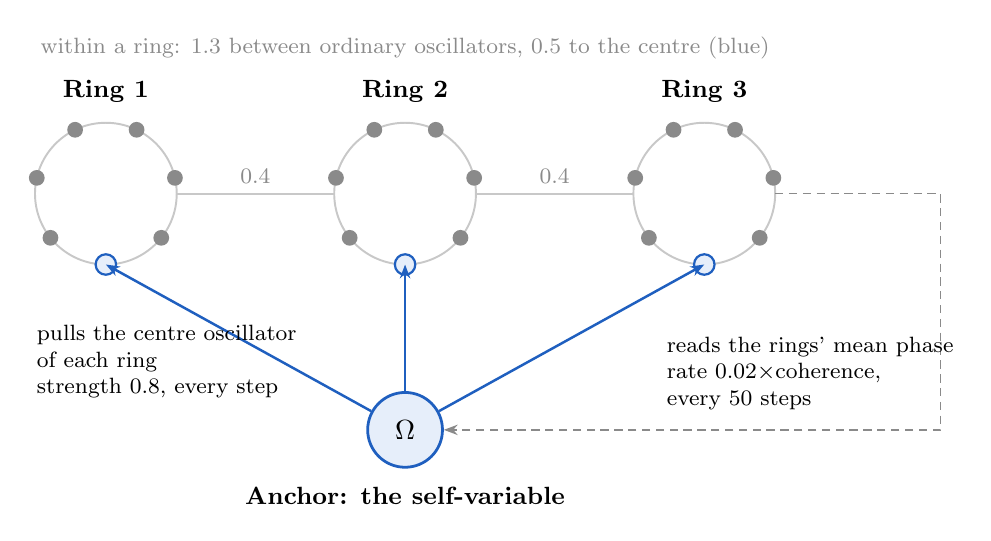
\begin{tikzpicture}[font=\small]
\def\R{0.9}
\foreach \c/\x in {1/0,2/3.8,3/7.6}{
  \draw[lg,line width=0.7pt] (\x,0) circle (\R);
  \foreach \k in {0,...,6}{ \pgfmathsetmacro{\a}{-90+\k*360/7}
    \ifnum\k=0 \fill[fillacc,draw=acc,line width=0.8pt] (\x,0)++(\a:\R) circle (0.13); \coordinate (c\c) at ($(\x,0)+(\a:\R)$);
    \else \fill[gry] (\x,0)++(\a:\R) circle (0.1); \fi}
  \node[font=\small\bfseries] at (\x,1.3) {Ring \c};}
\draw[lg,line width=0.7pt] (0.9,0)--(2.9,0) node[midway,above,font=\footnotesize,text=gry]{0.4};
\draw[lg,line width=0.7pt] (4.7,0)--(6.7,0) node[midway,above,font=\footnotesize,text=gry]{0.4};
\node[font=\footnotesize,text=gry,align=center] at (3.8,1.85) {within a ring: 1.3 between ordinary oscillators, 0.5 to the centre (blue)};
\node[circle,draw=acc,fill=fillacc,line width=1pt,minimum size=0.95cm,font=\bfseries] (om) at (3.8,-3.0) {$\Omega$};
\node[font=\small\bfseries,below=3pt of om] {Anchor: the self-variable};
\foreach \c in {1,2,3}{\draw[aarr] (om) -- (c\c);}
\node[align=left,font=\footnotesize,anchor=north west] at (-1.0,-1.55) {pulls the centre oscillator\\of each ring\\strength 0.8, every step};
\draw[arr,dash pattern=on 3pt off 2pt] (8.5,0) -- (10.6,0) -- (10.6,-3.0) -- (om.east);
\node[align=left,font=\footnotesize,anchor=north west] at (7.0,-1.7) {reads the rings' mean phase\\rate $0.02\times$coherence,\\every 50 steps};
\end{tikzpicture}
\end{document}
